\documentclass[11pt]{article}
\usepackage[scaled=0.92]{helvet}
\usepackage{geometry}
\geometry{letterpaper,tmargin=1in,bmargin=1in,lmargin=1in,rmargin=1in}
\usepackage[parfill]{parskip} % Activate to begin paragraphs with an empty line rather than an indent %\usepackage{graphicx}
\usepackage{amsmath,amssymb, mathrsfs, dsfont}
\usepackage{tabularx}
\usepackage[font=footnotesize,labelfont=bf]{caption}
\usepackage{graphicx}
\usepackage{xcolor}
%\usepackage[linkbordercolor ={1 1 1} ]{hyperref}
%\usepackage[sf]{titlesec}
\usepackage{natbib}
\usepackage{../../Tianpei_Report}

%\usepackage{appendix}
%\usepackage{algorithm}
%\usepackage{algorithmic}

%\renewcommand{\algorithmicrequire}{\textbf{Input:}}
%\renewcommand{\algorithmicensure}{\textbf{Output:}}



\begin{document}
\title{Lecture 4: Vector Fields}
\author{ Tianpei Xie}
\date{Oct. 13th., 2022}
\maketitle
\tableofcontents
\newpage
\section{Vector field on Euclidean space and on surface}
\subsection{Field of directions and vector field}
\begin{itemize}
\item \begin{definition}
A \underline{\emph{\textbf{vector field}}} $\mb{w}$ in an open set $U$ of Euclidean space $\bR^{2}$ is a map which assign to each $q\in U$ a vector $\mb{w}(q)\in \bR^{2}$. The vector field is said to be \emph{differentiable} if writing $q=(x,y)$ and $\mb{w}(q)= (a(x,y), b(x,y))$, the functions $a,b$ are differentiable function in $U$.
\end{definition}

\begin{figure}[htb]
\centering
\begin{minipage}{0.5\linewidth}
 \centerline{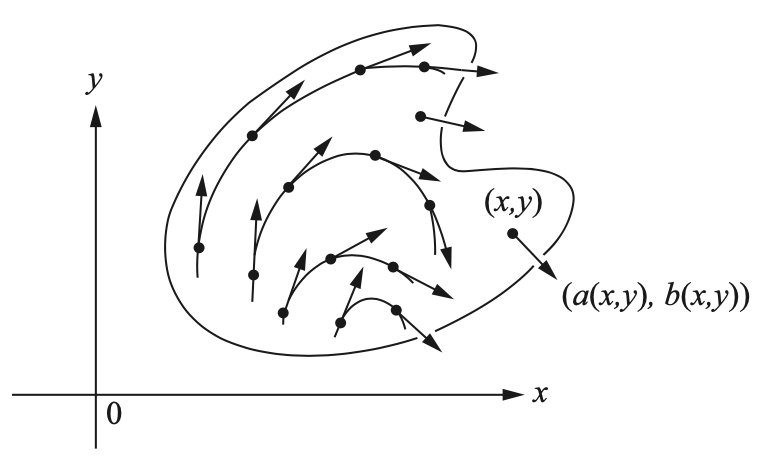
\includegraphics[scale = 0.5]{vector_fields.png}}
\end{minipage}
\caption{\scriptsize
\textbf{A vector field}}
\label{fig: vector_fields}
\end{figure}

\item \begin{definition}
A \emph{\textbf{(tangent) vector field}} $\mb{w}$ in an open set $U \subset \cS$ of a regular surface $\cS$ is a correspondence which assigns to each $p\in U$ a vector $\mb{w}(p) \in T_{p}S$. The vector field $\mb{w}$ is \emph{differentiable} at $p\in U$ if, for some parameterization $\mb{x}(u,v)$ at $p$, the functions $a(u,v)$ and $b(u,v)$ given by 
\begin{align*}
\mb{w}(p) &= a(u,v)\mb{x}_{u} + b(u,v)\mb{x}_{v}
\end{align*}
are differentiable functions at $p$; it is clear that this definition does not depends on the choice of $\mb{x}$. 
\end{definition}

\item  \begin{definition}
A \emph{\textbf{trajectory}} of a vector field $\mb{w}$ is a differentiable parameterized curve $\alpha(t)= (x(t), y(t)), t\in I$ such that $\alpha'(t) = \mb{w}(\alpha(t))$. 
\end{definition}

\item The vector field $\mb{w}$ determines \emph{a system of differential equations},
\begin{align*}
\frac{dx}{dt} &= a(x,y), \\
\frac{dy}{dt} &= b(x,y),
\end{align*}
and that a trajectory of $\mb{w}$ is a solution to the above system of equations.


\item \begin{theorem}\label{thm: unique_trajectory_1}
Let $\mb{w}$ be a vector field in an open set $U\subset \bR^{2}$. Given $p\in U$, there exists a trajectory $\alpha: I\rightarrow U$ of $\mb{w}$, i.e. $\alpha'(t) = \mb{w}(\alpha(t)), t\in I$ with $\alpha(0)=p$. This trajectory is unique in the following sense: Any other trajectory $\beta: J \rightarrow U$ with $\beta(0)=p$ agrees with $\alpha$ in $I\cap J$.
\end{theorem}
This gives the existence and uniqueness of trajectory in local neighborhood. 

\begin{figure}[htb]
\centering
\begin{minipage}{0.6\linewidth}
 \centerline{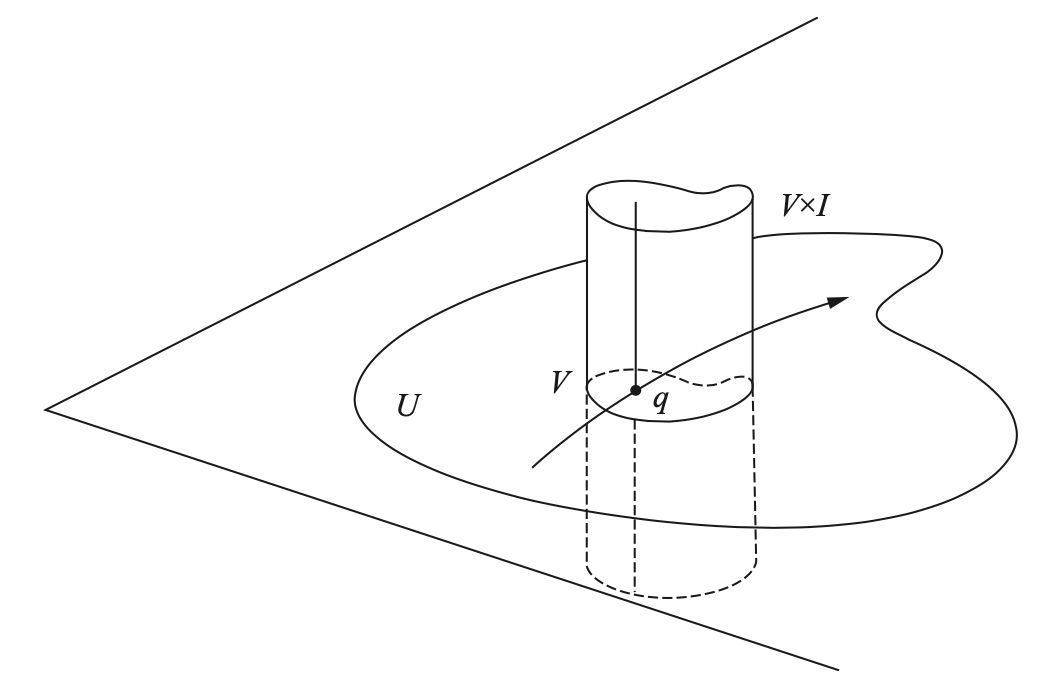
\includegraphics[scale = 0.5]{local_flow.png}}
\end{minipage}
\caption{\scriptsize
\textbf{All trajectories which pass $p$ in a neighborhood $V$ can be represented by $\alpha$}}
\label{fig: local_flow}
\end{figure}


\item \begin{theorem}\label{thm: unique_trajectory_2}
Let $\mb{w}$ be a vector field in an open set $U\subset \bR^{2}$. Given $p\in U$, there exists a neighborhood $V\subset U$ of $p$, an interval $I$, and a mapping $\alpha: V\times I \rightarrow U$ such that 
\begin{itemize}
\item For a fixed $p\in V$, the curve $\alpha(p, t), t\in I$, is the trajectory of $\mb{w}$ passing through $p$; that is,
\begin{align*}
\alpha(q, 0)= p, \quad \partdiff{\alpha}{t}(p,t) = \mb{w}\paren{\alpha(p,t)}
\end{align*}

\item $\alpha$ is differentiable. 
\end{itemize}
\end{theorem}
This means that the trajectory depends differentiable on initial point $p$. 

Geometrically Theorem \ref{thm: unique_trajectory_2} means that all trajectories which pass, for $t = 0$, in a certain neighborhood $V$ of $p$ may be "collected" into a single differentiable map. It is in this sense that we say that the trajectories depend differentiably on $p$.

\item \begin{definition}
The collection of trajectories $\alpha(q,t)$ passing through a neighborhood $V$ of $p$ is called a \emph{\textbf{(local) flow}} of $\mb{w}$ at $p$.
\end{definition}

\item Given the parameterization $\mb{x}(u,v)$ at $p$, the differentiable vector field $\mb{w}$ and the curve $\alpha(t) = \mb{x}(u(t), v(t))$ on $\cS$ with $\alpha(0)=p$, $\dot{\alpha}(0)= \mb{y}$, the vector field can be represented as 
\begin{align}
\mb{w}(t) &= a(u(t), v(t))\mb{x}_{u} + b(u(t), v(t))\mb{x}_{v} \nonumber\\
&= a(t)\mb{x}_{u} + b(t)\mb{x}_{v} \label{eqn: diff_vec_field}
\end{align}

\item \begin{lemma} (\textbf{The existence of first integral})\\
Let $\mb{w}$ be a vector field in an open set $U\subset \bR^{2}$ and let $p\in U$ such that $\mb{w}(p)\neq 0$. Then there exists a neighborhood $W\subset U$ of $p$ and a differentiable function $f: W\rightarrow \bR$ such that $f$ is \textbf{constant along each trajectory} of $\mb{w}$ and $df_{q}\neq 0$ for all $q\in W$.
\end{lemma}
\begin{proof}
Choose the Cartesian coordinate system in $\bR^{2}$ such that $p=(0,0)$ and $\mb{w}(p)$ is in direction of $x-$axis. Let the $\alpha: V\times I\rightarrow U$ be a local flow at $p$, $V\subset U, t\in I$, and let the $\hat{\alpha}$ be the restriction of $\alpha$ to the rectangle
$$ (V\times I)\cap \set{(x,y,t), x=0}  $$


By definition of the local flow, $d\hat{\alpha}_{p}$ maps the unit vector of the $t$ axis into $\mb{w}$ and maps the unit vector of $y$-axis into itself. Thus $d\hat{\alpha}_{p}\neq 0$. It follows that there exists a neighborhood $W\subset U$ of $p$, where $\hat{\alpha}^{-1}$ is defined and differentiable. The projection of $\hat{\alpha}^{-1}(x,y)$ onto the $y-$axis is a differentiable function $\xi = f(x,y)$, which has the same value $\xi$ for all points of the trajectory passing through $(0,\xi)$.

In other word, note that $\hat{\alpha}(0,y,t)$ is the point obtained by "walking" in the trajectory of $(0,y)$ an time $t$. On the other hand, $\hat{\alpha}^{-1}(x,y)$ are the points of the form $(0,y',t)$ for some $y'$ and some $t\in I$. The projection of $\hat{\alpha}^{-1}(x,y)$ onto the $y-$axis is the intersection of the trajectory passing through $(x,y)$ with the $y-$axis. By the uniqueness of the trajectory, if you take $(x,y)$ and $(x_1,y_1)$ in the same trajectory, they must pass through the same position $y$-axis, so the function $\hat{\alpha}^{-1}(x,y)$ is constant on trajectories.


Since $d\hat{\alpha}_{p}\neq 0$, $W$ may be taken sufficiently small so that $df_{q}\neq 0$ for all $q\in W$. $f$ is the function we required.  \QEDA
\end{proof}


\item \begin{definition}
The function $f: W\rightarrow \bR$ above is called a \emph{(local) first integral of a vector field} of $\mb{w}$ in a neighborhood $W$ of $p$.  In other word, for $f$ to be \emph{\textbf{\underline{the first integral} of vector field}} $\mb{w}$, $\alpha(t)$ be the trajectory of the vector field, then 
\begin{align*}
\frac{df(\alpha(t))}{dt} &= a(u,v)\partdiff{f}{u} + b(u,v)\partdiff{f}{v} \\
& \equiv \mb{w}(f)= 0
\end{align*}
\end{definition}
In other word, the \textbf{curve} $f(\alpha(t)) = const$ is seen as \textbf{\emph{one solution}} for the system of differential equations.

\begin{figure}[tb]
\centering
\begin{minipage}{0.6\linewidth}
 \centerline{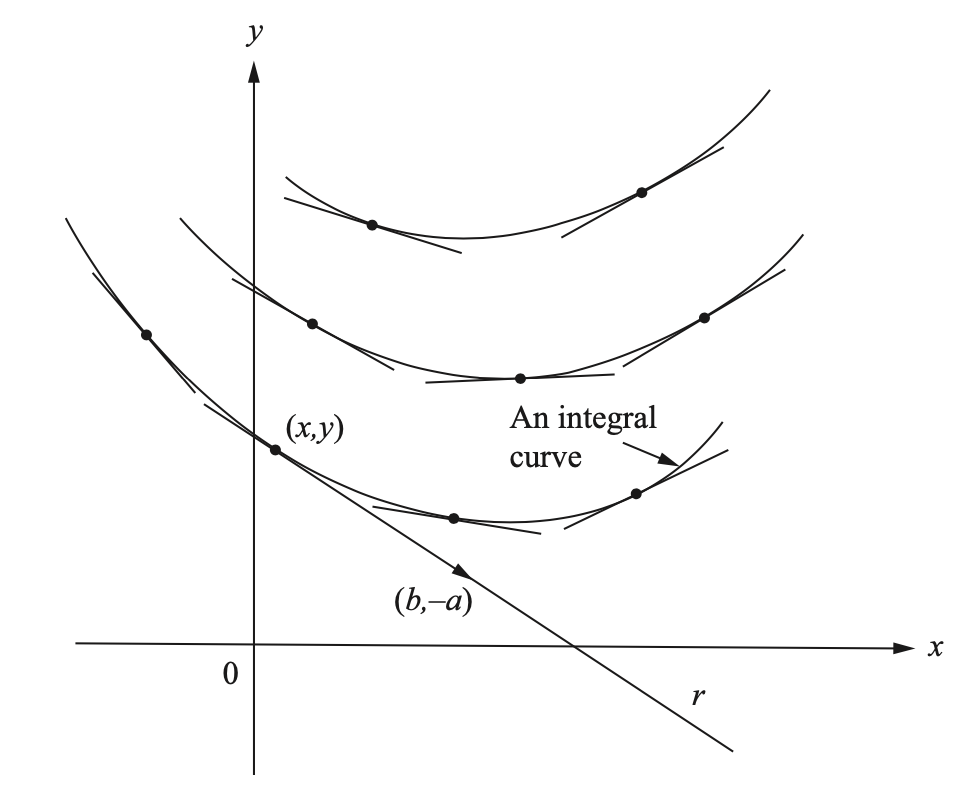
\includegraphics[scale = 0.5]{integral_curve.png}}
\end{minipage}
\caption{\scriptsize
\textbf{An integral curve of differential equations}}
\label{fig: integral_curve}
\end{figure}

\item \begin{definition}
A \emph{\textbf{field of directions}} $r$ is an open set $U\subset \bR^{2}$ is a correspondence which assigns to each $p\in U$ a \emph{\textbf{line}} $r(p)$ in $\bR^{2}$ passing through $p$. 

$r$ is said to be \emph{\textbf{differentiable}} at $p\in U$ if there exists \emph{nonzero differentiable vector field} $\mb{w}$ defined in a neighborhood $V\subset U$ of $p$, such that for each $q\in V$, $\mb{w}(q)\neq 0$ is a \emph{\textbf{basis}} of $r(q)$; $r$ is \emph{differentiable} in $U$, if it is \emph{differentiable} in every $p\in U$.
\end{definition}

\begin{definition}
In differential equations, a \emph{\textbf{field of directions}} is given by 
\begin{align*}
a(x,y)\frac{dx}{dt} + b(x,y)\frac{dy}{dt} &= 0
\end{align*}
The above form is also called \textbf{\emph{$1-$form differentials}}.
\end{definition}


\begin{figure}[tb]
\centering
\begin{minipage}{0.6\linewidth}
 \centerline{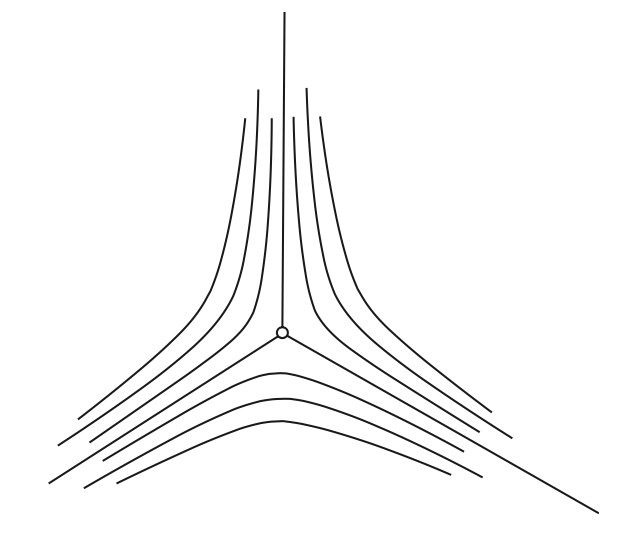
\includegraphics[scale = 0.5]{field_of_directions.png}}
\end{minipage}
\caption{\scriptsize
\textbf{Field of directions and the integral curve.}}
\label{fig: field_of_directions}
\end{figure}

\item Note that for each differentiable $\mb{w}$ in $U$ there exists a differentiable field of directions $r$ with $r(p) = \text{line generated by }\mb{w}(p)$.

\item \begin{definition}
A \emph{regular} \emph{connected} curve $\cC\subset U$ is an \emph{\textbf{integral curve of a field of directions}} $r$ defined in $U$ if $r(q)$ is the \emph{\textbf{tangent line}} to $\cC$ at $q$ for all $q\in \cC$. 
\end{definition}
It is clear that given $r$ in $U$, there passes, for each $q\in U$ an integral curve of $r$.

\item The \emph{\textbf{difference}} between \emph{field of directions} and the \emph{vector field} is that for $\mb{w}_{2} = \lambda\mb{w}_{1}$ with $\lambda\neq 0$ constant, they corresponds to the \emph{\textbf{same field of direction}} $r$ (i.e. up to scale). 

\textbf{Conversely}, if two vectors belong to the same straight line passing through $p$ they are considered equivalent.  Thus for every $p\in U$, $r(p) = (r_{1}, r_{2})$ with $r_{1}, r_{2}$ being two real numbers and $ (r_{1}, r_{2}) \sim  (\lambda r_{1}, \lambda r_{2})$ 
\end{itemize}

\subsection{Vector fields in local coordinates and derivative of functions}
\begin{itemize}
\item \begin{theorem}\label{thm: local_parm_vec_field}
Let $\mb{w}_{1}, \mb{w}_{2}$ are two vector fields in an open subset $U\subset \cS$, which are linearly independent at some point $p\in U$. Then it is possible to \textbf{parameterize} a neighborhood $V\subset U$ of $p$ in a way that for each $q\in V$ the coordinate lines of this parameterization passing through $q$ are \textbf{tangent} to the lines determined by $\mb{w}_{1}(q)$ and $\mb{w}_{2}(q)$.
 \end{theorem}
 (\emph{Note that not necessary to be the tangent line.})
 \begin{proof}
 Let $W$ be a neighborhood of $p$ where the first integrals $f_{1}$ and $f_{2}$ of $\mb{w}_{1}, \mb{w}_{2}$, respectively, are defined. Define a map $\varphi: W\rightarrow \bR^{2}$ as
 \begin{align*}
 \varphi(q) &= (f_{1}(q), f_{2}(q)), \quad q\in W.
 \end{align*}
 Since $f_{1}$ is constant on the trajectory of $\mb{w}_{1}$ and $df_{1}\neq 0$, we have at $p$
 \begin{align*}
 d\varphi_{p}(\mb{w}_{1}) &= ((df_{1})_{q}(\mb{w}_{1}), (df_{2})_{q}(\mb{w}_{1})) = (0, a),
 \end{align*}
 where $a=  (df_{2})_{q}(\mb{w}_{1})\neq 0$, since $\mb{w}_{1}, \mb{w}_{2}$ are linearly independent. Similarly, see that
  \begin{align*}
 d\varphi_{p}(\mb{w}_{2}) &= (b,0),
 \end{align*}
 where $b = (df_{1})_{q}(\mb{w}_{2})\neq 0$. It follows that $ d\varphi_{p}\neq 0$ and hence $\varphi$ is a local diffeomorphism. There exist, therefore, a neighborhood $\bar{U}\subset \bR^{2}$ of $\varphi(p)$ which is mapped diffeomorphically by $\mb{x} = \varphi^{-1}$ onto a neighborhood $V = \mb{x}(\bar{U})$ of $p$; that is, $\mb{x}$ is a parameterization of $\cS$ at $p$, whose coordinate curve is given by 
 \begin{align*}
 f_{1}(q) = const. && f_{2}(q) = const.
 \end{align*}
 are tangent at $q$ to the lines determined by $\mb{w}_{1}(q)$ and $\mb{w}_{2}(q)$.\QEDA
 \end{proof}
 
 \item \begin{corollary}\label{cor: local_parm_field_dir}
 Given two fields of directions $r_{1}, r_{2}$ in an open set $U\subset \cS$ such that at $p\in U$, $r_{1}(p)\neq r_{2}(p)$, there exists a \textbf{parameterization} $\mb{x}$ in a neighborhood of $p$ such that the \textbf{coordinate curves} of $\mb{x}$ are the \textbf{integral curves} of $r_{1}, r_{2}$.
 \end{corollary}
 
 \item \begin{corollary}\label{cor: local_parm_field_dir}
 (\textbf{The existence of the orthogonal parameterization}). \\
For all $p\in U$, there exists a \textbf{parameterization} $\mb{x}(u,v)$ is a neighborhood $V$ of $p$ such that the coordinate curve $u=const.$ and $v=const.$ intersects \textbf{orthogonally} for each $q\in V$ (such that $\mb{x}$ is called an \textbf{orthogonal parameterization}).
 \end{corollary}
 
 \item It thus represent the \textbf{basis vector field} as $\partdiff{}{u}$ and $\partdiff{}{v}$, and
 \begin{align*}
 \mb{w}(u,v) & = a(u,v)\partdiff{}{u} + b(u,v)\partdiff{}{v}
 \end{align*}

\item \begin{corollary}
Let $p\in \cS$ be a hyperbolic point of $\cS$.Then it is possible to parametrize a neighborhood of $p$ in such a way that the coordinate curves of this parametrization are the \textbf{asymptotic curves} of $\cS$.
\end{corollary} 

\item \begin{corollary}
Let $p\in \cS$ be a non-umbilical point of $\cS$.Then it is possible to parametrize a neighborhood of $p$ in such a way that the coordinate curves of this parametrization are the \textbf{lines of curvature} of $\cS$.
\end{corollary} 

 

\item  \begin{definition}
Define \emph{the \underline{\textbf{derivative} $\mb{w}(f)$ of a differentiable function} $f: U\subset \cS \rightarrow \bR$ relative to a \underline{\textbf{vector field}}} $\mb{w}$ in $U$ by 
\begin{align*}
\mb{w}(f)(q) &= \rlat{\frac{d}{dt}\paren{f\circ \alpha}}{t=0},\quad q\in U
\end{align*}
where $\alpha: I\rightarrow \cS$ is the \emph{\textbf{trajectory of}} $\mb{w}$ passing through $q$ such that $\alpha(0) = q, \alpha'(0)=\mb{w}(q)$.
\end{definition}

\item Thus the vector field $\mb{w}$ can also be considered as a \emph{\underline{\textbf{differential operator}} on \textbf{space of continuous functions}} $\mathbb{C}^{\infty}$ as $\mb{w}: \mathbb{C}^{\infty} \rightarrow \mathbb{C}^{\infty}$ as $$\mb{w}(f) = \text{directional derivative of }f\text{ along trajectory }\alpha \text{ of }\mb{w}.$$ 
 Then 
 \begin{align*}
 \mb{w}(f) &= \paren{a(u,v)\partdiff{}{u} + b(u,v)\partdiff{}{v}}(f)\\
 &= a(u,v)\partdiff{f}{u} + b(u,v)\partdiff{f}{v}
 \end{align*}
 
 \item The composition of two vector fields $\mb{w,v}$ together gives 
 \begin{align*}
\mb{w}\mb{v}(fg)\equiv \mb{w}\paren{\mb{v}(fg)} &= \mb{w}\paren{\mb{v}(f)g}+ \mb{w}\paren{f\mb{v}(g)}\\
 &= \mb{w}\paren{\mb{v}(f)}g+  \mb{v}\paren{f}\mb{w}\paren{g}+ \mb{w}\paren{f}\mb{v}(g)+ f\mb{w}\paren{\mb{v}\paren{g}}\\
 \mb{v}\mb{w}(fg) &=
 \mb{v}\paren{\mb{w}(f)}g+  \mb{w}\paren{f}\mb{v}\paren{g}+ \mb{v}\paren{f}\mb{w}(g)+ f\mb{v}\paren{\mb{w}\paren{g}}\\
 \brac{\mb{w\,v} - \mb{v\,w}}(fg) &= \paren{\brac{\mb{w\,v} - \mb{v\,w}}(f)}g + f\paren{\brac{\mb{w\,v} - \mb{v\,w}}(g)}\\
 \brac{\mb{w},\, \mb{v}}(fg) &= \paren{\brac{\mb{w},\, \mb{v}}(f)}g + f\paren{\brac{\mb{w},\, \mb{v}}(g)}
 \end{align*}
 where the operator
 \begin{align*}
 \brac{\mb{w},\, \mb{v}} &\equiv \brac{\mb{w\,v} - \mb{v\,w}}
 \end{align*}
 is called the \emph{\textbf{Lie bracket}}. 
\end{itemize}



\newpage
\bibliographystyle{plainnat}
\bibliography{book_reference.bib}
\end{document}